\documentclass[12pt, a4paper]{article}
\usepackage[utf8]{inputenc}
\usepackage[russian]{babel}
\usepackage[pdftex]{graphicx, color}
\usepackage{amsmath}
\usepackage{amsfonts}
\usepackage{amssymb}
\usepackage{amsthm}
\usepackage[left=2cm,right=1.5cm,top=1.5cm,bottom=2cm]{geometry}
\usepackage{indentfirst}
\usepackage{hyperref}

\usepackage{setspace}
\onehalfspacing
\graphicspath{{pic/}}

\begin{document}

	\thispagestyle{empty}

	\begin{singlespace}
	\begin{titlepage}
		\begin{center}
			
\includegraphics[height = 3cm]{msu.png}

			{\scshape Московский государственный университет имени М.~В.~Ломоносова}\\
			Факультет вычислительной математики и кибернетики\\
			\centerline{\hfill\hrulefill\hrulefill\hrulefill\hrulefill\hfill}

			\vfill

			{\LARGE Отчет к первому заданию практикума на ЭВМ: \\ Изучение Python, NumPy, SVN}

			\vspace{1cm}

		\end{center}

		\vfill
		\begin{flushright}
			\textit{Студент 3 курса ВМК (317 группа):}\\
				Оспанов А.М.

			\vspace{5mm}

		\end{flushright}

		\vfill

		\begin{center}
		Москва, 2014
		\end{center}
	\end{titlepage}
	\end{singlespace}

	\tableofcontents


	\newpage
	\section{Введение}
		Данный отчет написан к первому заданию практикума на ЭВМ 317 группы. Тема задания: Изучение Python, NumPy и SVN. Отчет написан студентом 317 группы -- Оспановым Аятом.

		В данной работе было решено 8 задач, каждый из которых имеет по три способа решения (кроме 1й задачи, который имеет 4 способа). Минимум имеется один векторизованный вариант и один невекторизованный вариант решения каждой из задач. Каждый вариант решения сравнивался на скорость работы (посредством \%timeit) и все варианты в одной задаче тестировались на правильность ответа (посредством unittest).

		В выполнении данной работы использовалась операционная система OS X 10.9. В качестве клиента SVN использовалась программа Versions (v. 1.3.0, OS X, shareware). Версия Python - 3.4.1, версия NumPy - 1.9.0


	\newpage
	\section{Основная часть}
		\subsection{Работа с SVN}

			\begin{center}
				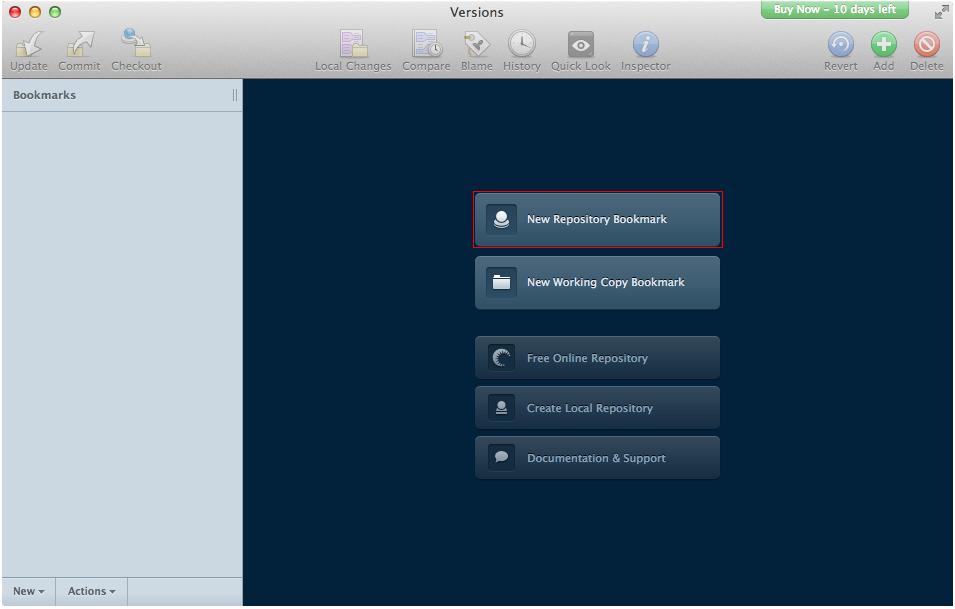
\includegraphics[height=10.5cm]{svn/svn_1.png}

				Открываем программу и видим главное окно. Нажимаем New Repository Bookmark \\
				~\newline
			\end{center}

			\begin{center}
				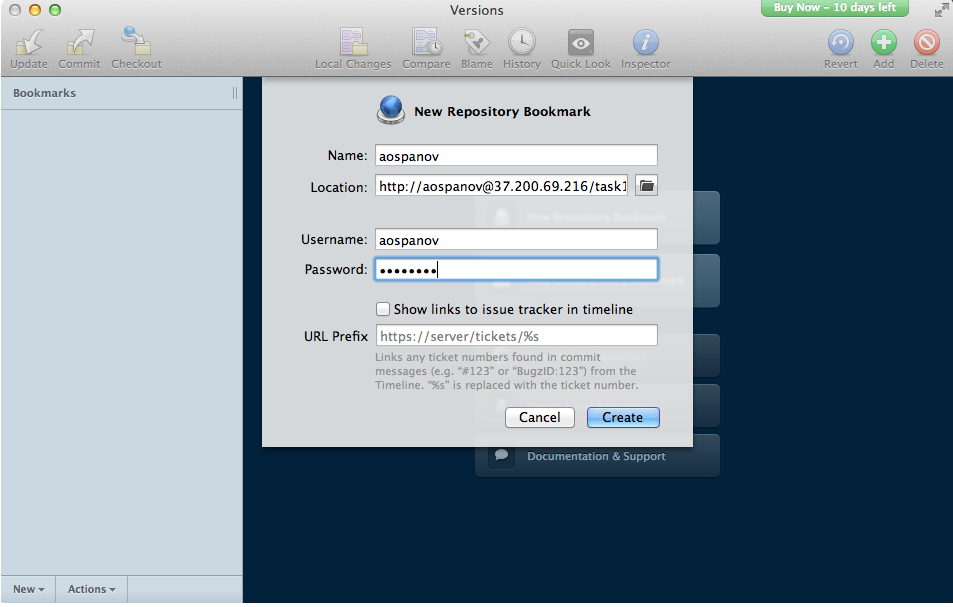
\includegraphics[height=10.5cm]{svn/svn_2.png}

				Далее выходит окошко для ввода адреса репозитория, логина и пароля \\

			\end{center}

			\begin{center}
				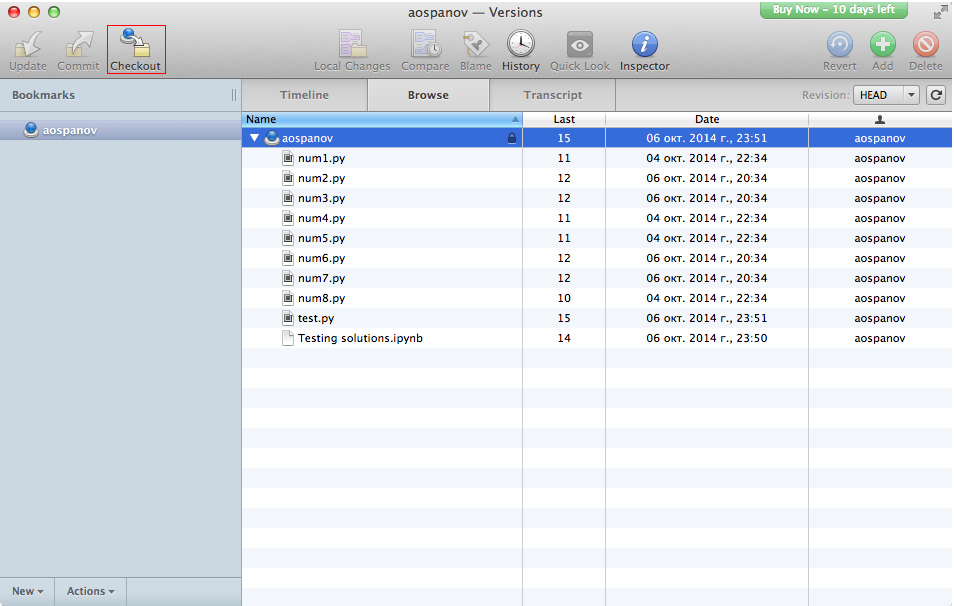
\includegraphics[height=10.5cm]{svn/svn_3.png}

				После открывается наш репозиторий. Делаем Checkout в нужную нам папку \\
				~\newline
			\end{center}

			\begin{center}
				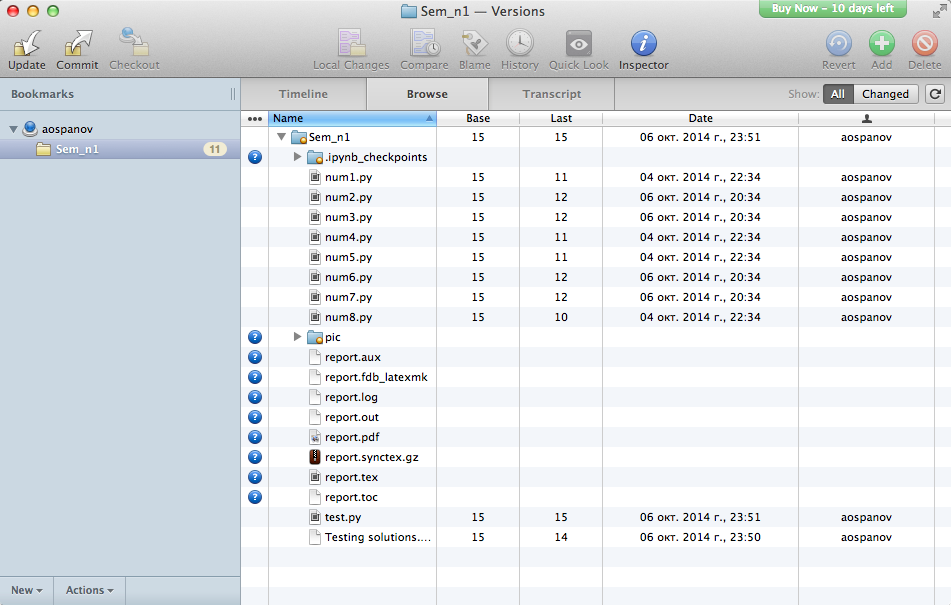
\includegraphics[height=10.5cm]{svn/svn_4.png}

				Видим файлы, которые в данный момент есть в папке + данные с репозитория \\
			\end{center}

			\begin{center}
				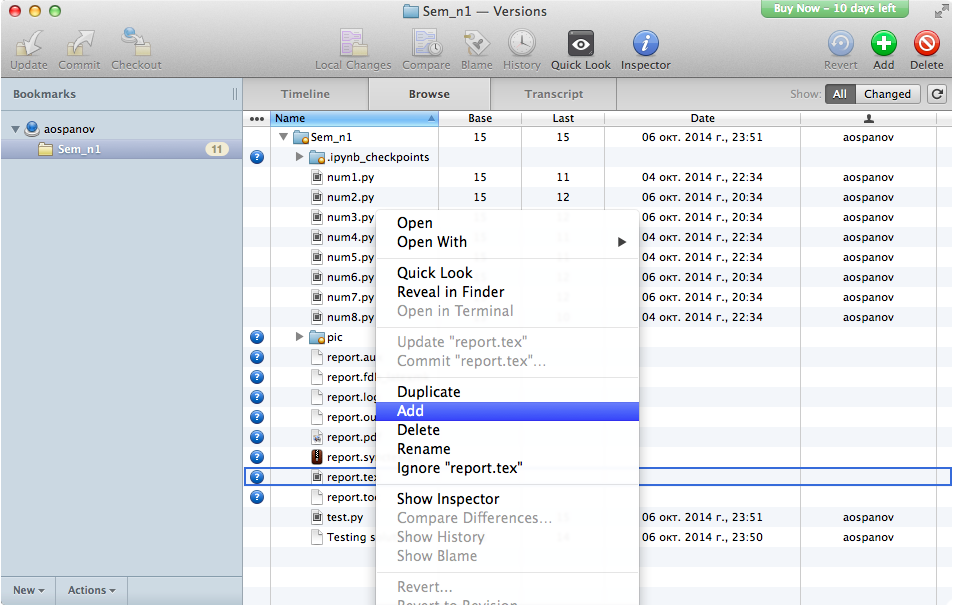
\includegraphics[height=10.5cm]{svn/svn_5.png}

				Нужные добавляем через "Add" \\
				~\newline
			\end{center}

			\begin{center}
				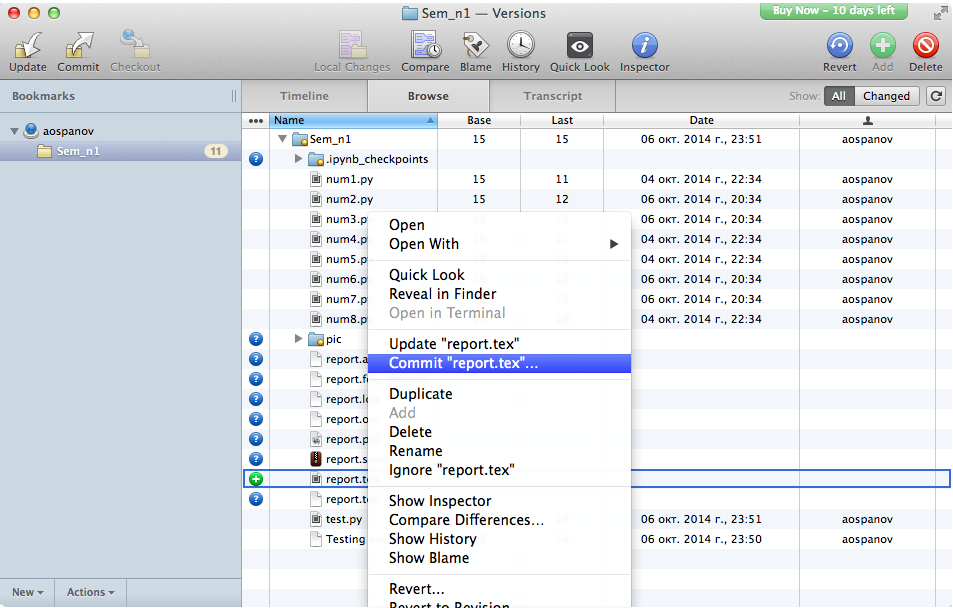
\includegraphics[height=10.5cm]{svn/svn_6.png}

				Затем нажимаем "Commit" \\
			\end{center}

			\begin{center}
				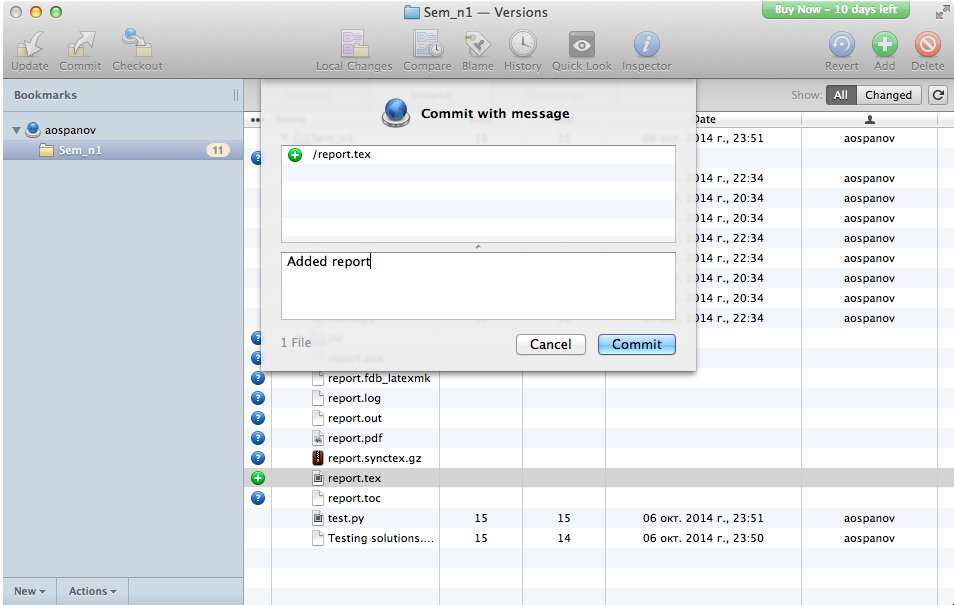
\includegraphics[height=10.5cm]{svn/svn_7.png}

				Пишем комментарий к коммиту и жмем "Commit" \\
				~\newline
			\end{center}

			\begin{center}
				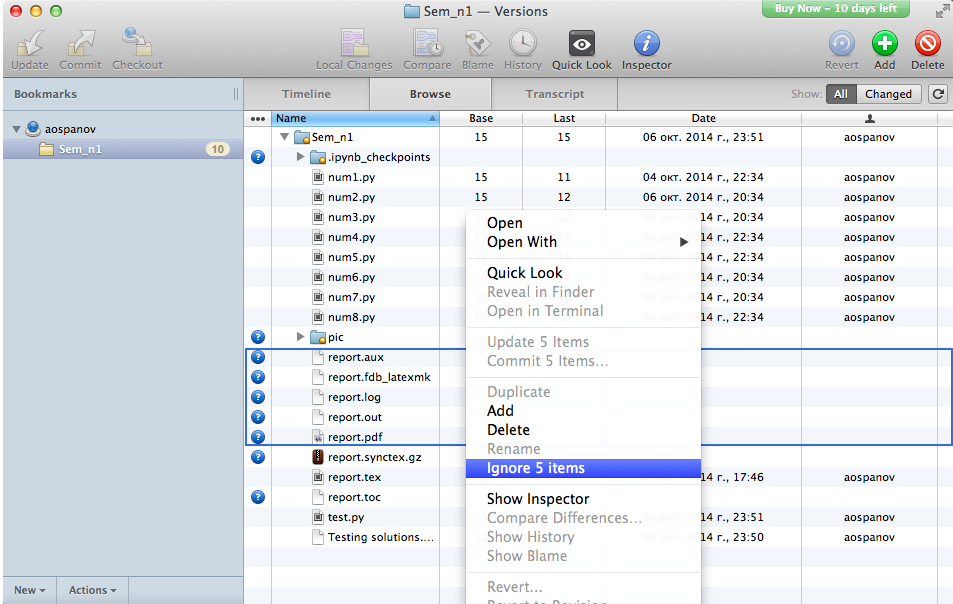
\includegraphics[height=10.5cm]{svn/svn_8.png}

				Ненужные файлы можно добавить в игнор-лист. Для этого выбираем файлы, которые хотим скрыть и нажимем "Ignore ..." \\
			\end{center}

			\begin{center}
				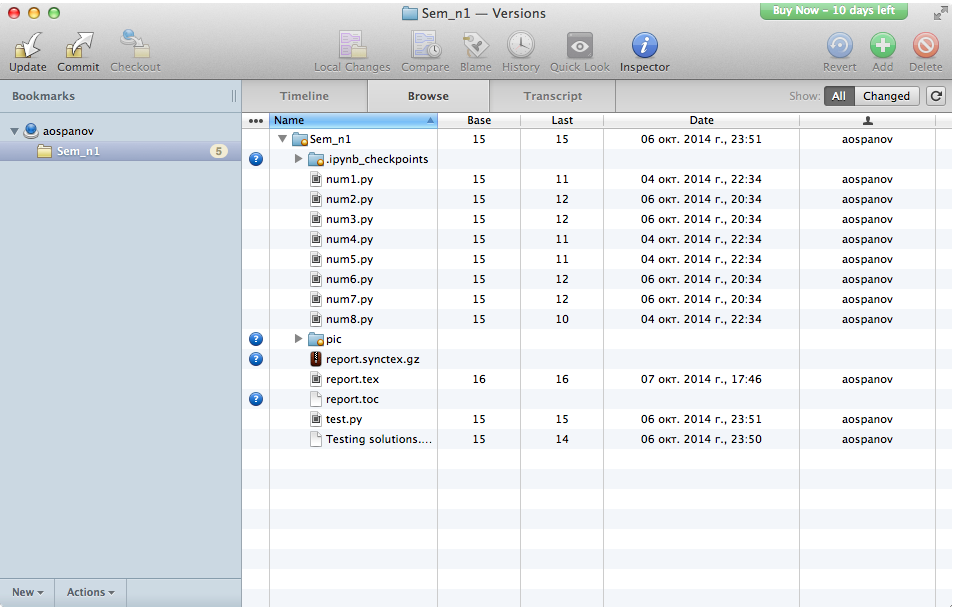
\includegraphics[height=10.5cm]{svn/svn_9.png}

				Видим, что они исчезли \\
				~\newline
			\end{center}

			\begin{center}
				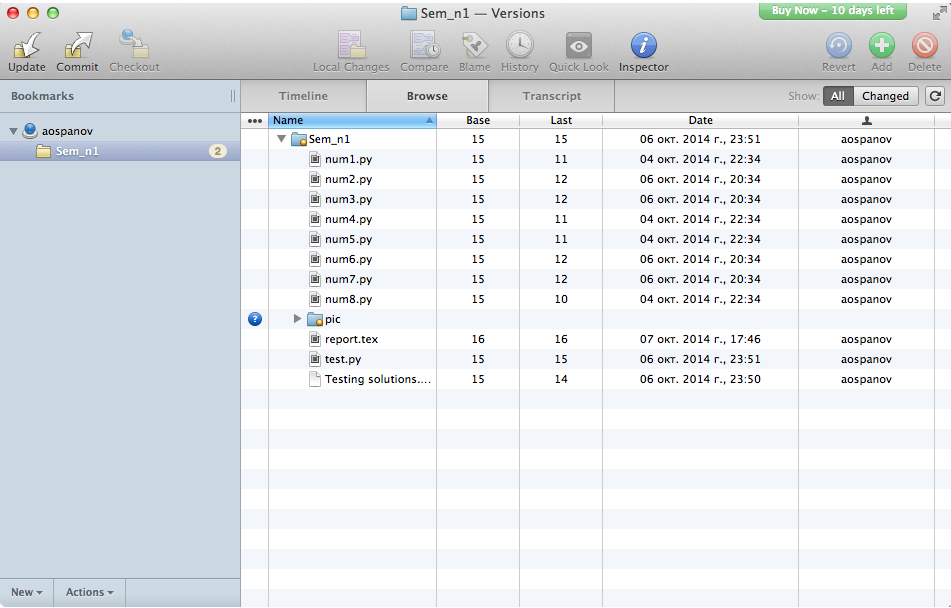
\includegraphics[height=10.5cm]{svn/svn_10.png}

				После всех манипуляций, получаем готовый к работе репозиторий \\
			\end{center}

			\begin{center}
				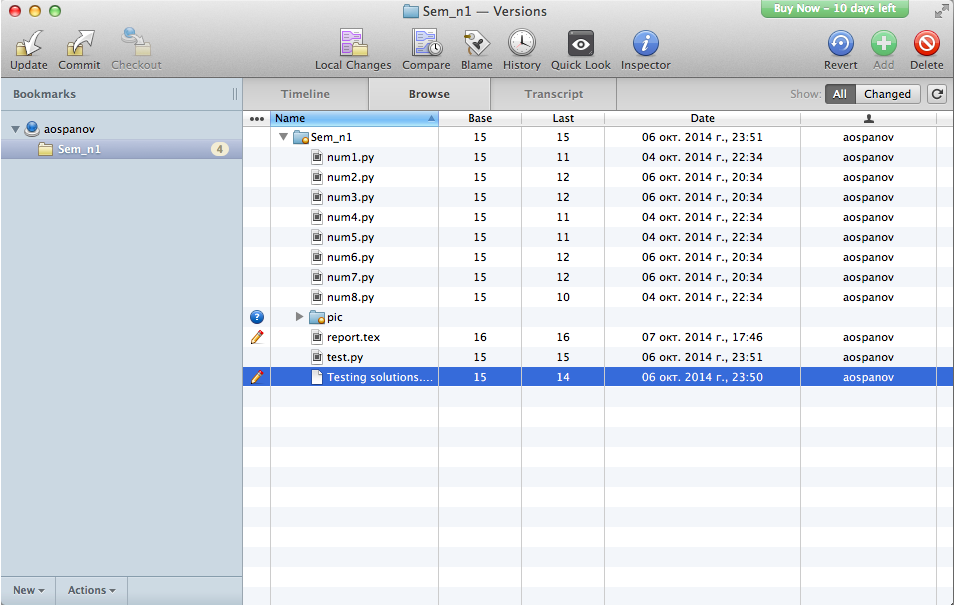
\includegraphics[height=10.5cm]{svn/svn_11.png}

				Попробуем изменить файлы. И видим, что измененные файлы отмечены значком карандашика. Их можно закоммитить, либо вернуть уже закоммиченную версию \\
				~\newline
			\end{center}

			\begin{center}
				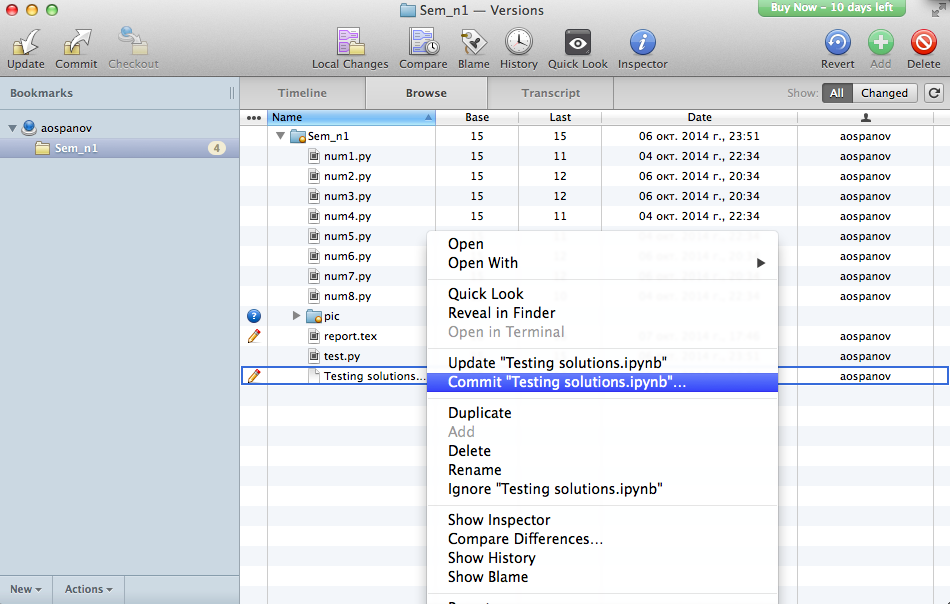
\includegraphics[height=10.5cm]{svn/svn_12.png}

				Давайте сделаем коммит. В контекстном меню нажимаем "Commit" \\
			\end{center}

			\begin{center}
				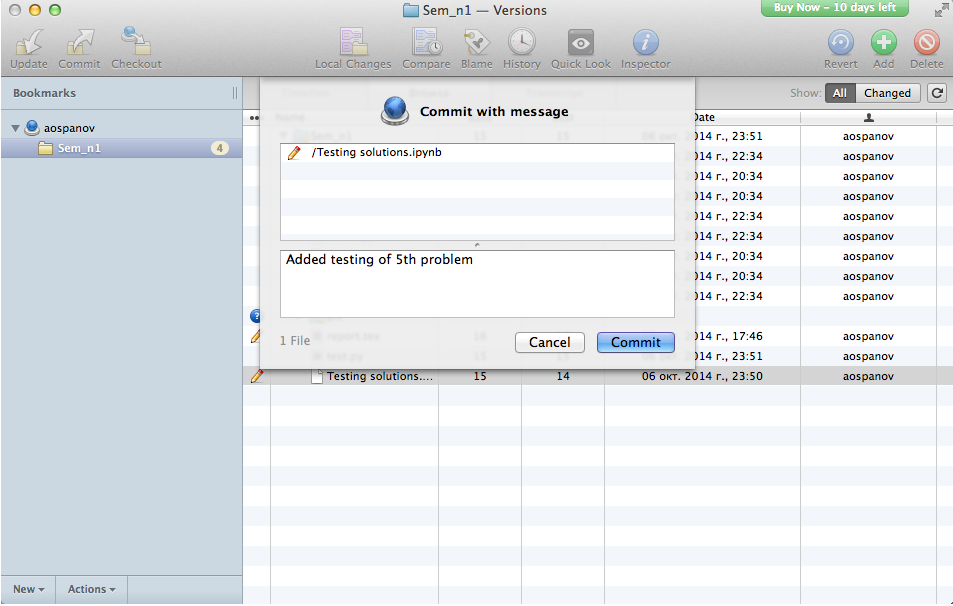
\includegraphics[height=10.5cm]{svn/svn_13.png}

				Далее вводим комментарий и коммитим \\
				~\newline
			\end{center}


			Вот так выполняется работа с SVN. Легко и просто!



		\newpage
		\subsection{Задача 1}

			{\bf Постановка задачи\\}

				Подсчитать произведение ненулевых элементов на диагонали прямоугольной матрицы. \\

				{\bf 1-й способ решения задачи\\}

				В первом способе решения задачи мы пробегаемся по диагонали матрицы и перемножаем все ненулевые элементы.

				Скорость выполнения данного способа от размера данных приведен в следующем графике:
				\begin{center}
					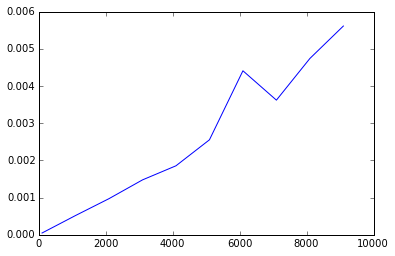
\includegraphics[height=7cm]{timeit/num1_ti1.png}
				\end{center}


			{\bf 2-й способ решения задачи\\}

				Во втором способе решения задачи (векторизованный) мы берем диагональ матрицы, берем ненулевые элементы и перемножаем их (все посредством NumPy функций).

				Скорость выполнения данного способа от размера данных приведен в следующем графике:
				\begin{center}
					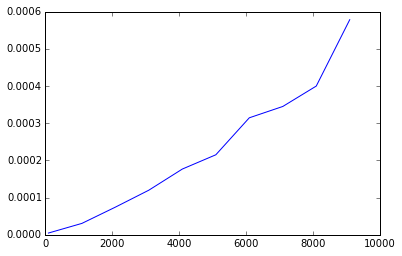
\includegraphics[height=7cm]{timeit/num1_ti2.png}
				\end{center}


			{\bf 3-й способ решения задачи\\}

				В третьем способе решения задачи мы пробегаемся по всей матрице и перемножаем все ненулевые элементы лежащие на диагонали.

				Скорость выполнения данного способа от размера данных приведен в следующем графике:
				\begin{center}
					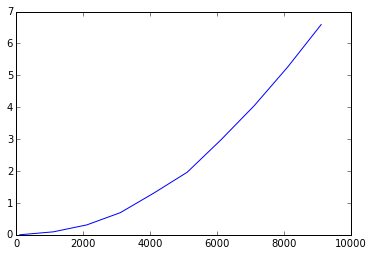
\includegraphics[height=7cm]{timeit/num1_ti3.png}
				\end{center}


			{\bf 4-й способ решения задачи\\}

				В четвертом способе решения первой задачи мы пробегаемся по матрице и присваиваем 1 к нулевым элементам и посредством NumPy перемножаем диагональные элементы.

				Скорость выполнения данного способа от размера данных приведен в следующем графике:
				\begin{center}
					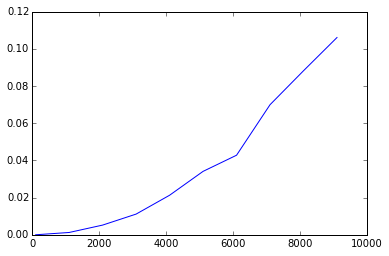
\includegraphics[height=7cm]{timeit/num1_ti4.png}
				\end{center}


			{\bf Сравнение скоростей работы\\}

				Как видно из графиков приведенных выше, самой быстрой оказался 2-й способ решения данной задачи. А самый медленный способ - 3-й способ, в чем можно убедится в следующем графике показывающих скорость работы всех методов:
				\begin{center}
					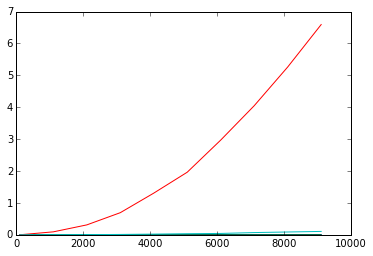
\includegraphics[height=7cm]{timeit/num1_ti1234.png}
				\end{center}



		\newpage
		\subsection{Задача 2}

			{\bf Постановка задачи\\}

				Дана матрица X и два вектора одинаковой длины i и j. Построить вектор np.array([X[i[0], j[0]], X[i[1], j[1]], . . . , X[i[N-1], j[N-1]]]) \\

				{\bf 1-й способ решения задачи\\}

				В первом способе решения задачи мы в цикле добавляем в новый массив элемент матрицы в нужном нам виде.

				Скорость выполнения данного способа от размера данных приведен в следующем графике:
				\begin{center}
					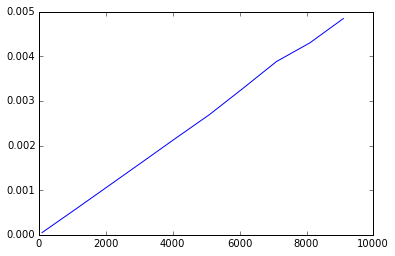
\includegraphics[height=7cm]{timeit/num2_ti1.png}
				\end{center}


			{\bf 2-й способ решения задачи\\}

				Во втором способе решения задачи мы делаем то же самое, что и в первом способе, но через list comprehension.

				Скорость выполнения данного способа от размера данных приведен в следующем графике:
				\begin{center}
					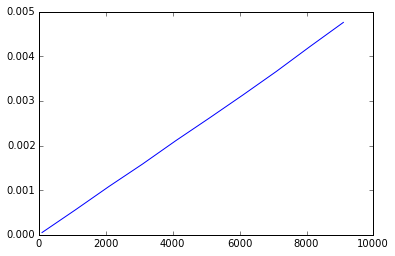
\includegraphics[height=7cm]{timeit/num2_ti2.png}
				\end{center}


			{\bf 3-й способ решения задачи\\}

				В третьем способе решения задачи мы используем индексацию NumPy.

				Скорость выполнения данного способа от размера данных приведен в следующем графике:
				\begin{center}
					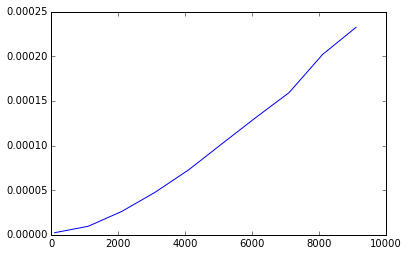
\includegraphics[height=7cm]{timeit/num2_ti3.png}
				\end{center}


			{\bf Сравнение скоростей работы\\}

				Как видно из графиков приведенных выше, самой быстрой оказался 3-й способ решения данной задачи. А 2-й и 3-й способы ведут себя примерно одинаково. Убедится в этом можно в следующем графике показывающих скорость работы всех методов:
				\begin{center}
					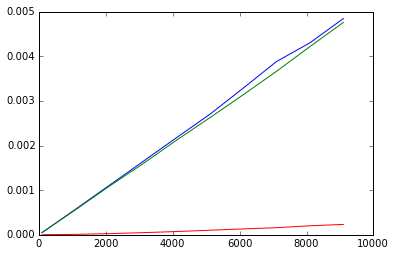
\includegraphics[height=7cm]{timeit/num2_ti123.png}
				\end{center}



		\newpage
		\subsection{Задача 3}

			{\bf Постановка задачи\\}

				Даны два вектора x и y. Проверить, задают ли они одно и то же мультимножество. \\

				{\bf 1-й способ решения задачи\\}

				Первый способ имеет невектаризованный вариант решения

				Скорость выполнения данного способа от размера данных приведен в следующем графике:
				\begin{center}
					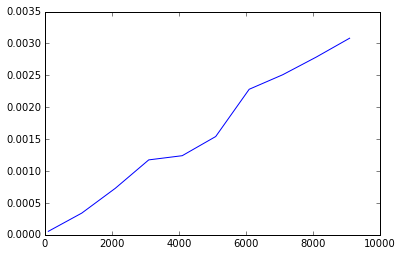
\includegraphics[height=7cm]{timeit/num3_ti1.png}
				\end{center}


			{\bf 2-й способ решения задачи\\}

				Во втором способе используются встроенные функции NumPy

				Скорость выполнения данного способа от размера данных приведен в следующем графике:
				\begin{center}
					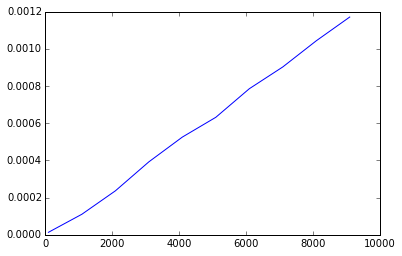
\includegraphics[height=7cm]{timeit/num3_ti2.png}
				\end{center}
				~\newline


			{\bf 3-й способ решения задачи\\}

				В третьем способе решения задачи мы используем двойной цикл.

				Скорость выполнения данного способа от размера данных приведен в следующем графике:
				\begin{center}
					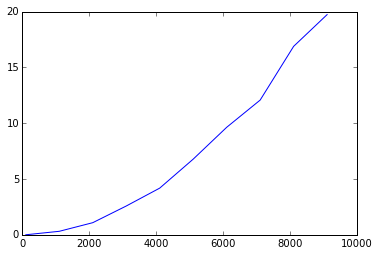
\includegraphics[height=7cm]{timeit/num3_ti3.png}
				\end{center}


			{\bf Сравнение скоростей работы\\}

				Как видно из графиков приведенных выше, самой быстрой оказался 2-й способ решения данной задачи. А самой медленной оказался 3-й способ, причем время работы очень высокое. Убедится в этом можно в следующем графике показывающих скорость работы всех методов:
				\begin{center}
					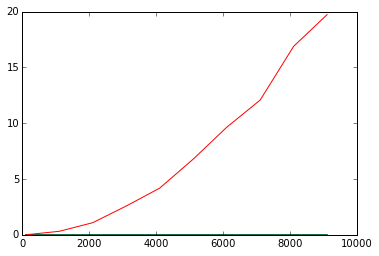
\includegraphics[height=7cm]{timeit/num3_ti123.png}
				\end{center}



		\newpage
		\subsection{Задача 4}

		% Задача 1
		% Способы решения задач и сравнение скоростей работы
			{\bf Постановка задачи\\}

				Найти максимальный элемент в векторе x среди элементов, перед которыми стоит нулевой \\

			{\bf 1-й способ решения задачи\\}

				Первый способ имеет невектаризованный вариант решения, использующий один цикл.

				Скорость выполнения данного способа от размера данных приведен в следующем графике:
				\begin{center}
					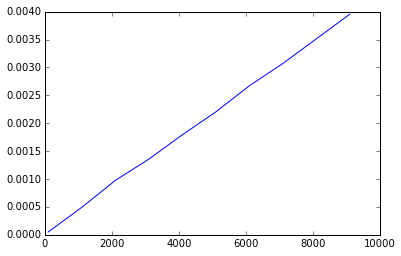
\includegraphics[height=7cm]{timeit/num4_ti1.png}
				\end{center}


			{\bf 2-й способ решения задачи\\}

				Во втором способе используются встроенные функции NumPy

				Скорость выполнения данного способа от размера данных приведен в следующем графике:
				\begin{center}
					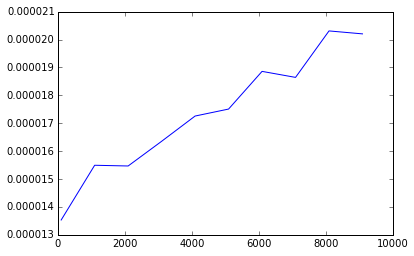
\includegraphics[height=7cm]{timeit/num4_ti2.png}
				\end{center}
				~\newline


			{\bf 3-й способ решения задачи\\}

				В третьем способе решения задачи мы используем двойной цикл.

				Скорость выполнения данного способа от размера данных приведен в следующем графике:
				\begin{center}
					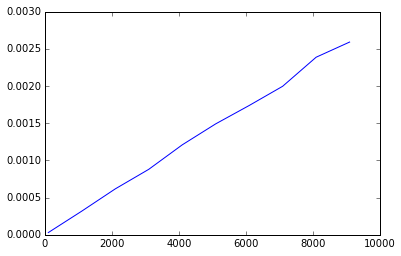
\includegraphics[height=7cm]{timeit/num4_ti3.png}
				\end{center}


			{\bf Сравнение скоростей работы\\}

				Как видно из графиков приведенных выше, самой быстрой оказался 2-й способ решения данной задачи. А самой медленной оказался 1-й способ, что является странным, ибо использовался одинарный цикл, вместо двойного в 3-ем способе. Убедится в этом можно в следующем графике показывающих скорость работы всех методов:
				\begin{center}
					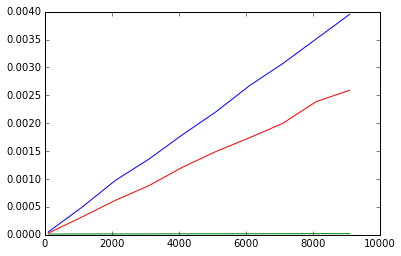
\includegraphics[height=7cm]{timeit/num4_ti123.png}
				\end{center}



		\newpage
		\subsection{Задача 5}

			{\bf Постановка задачи\\}

				Дан трехмерный массив, содержащий изображение, размера (height, width, numChannels), а также вектор длины numChannels. Сложить каналы изображения с указанными весами, и вернуть результат в виде матрицы размера (height, width). \\

			{\bf 1-й способ решения задачи\\}

				Первый способ имеет невектаризованный вариант решения, использующий матричное перемножение.

				Скорость выполнения данного способа от размера данных приведен в следующем графике:
				\begin{center}
					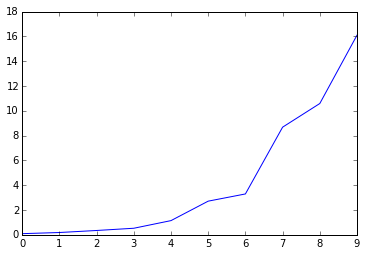
\includegraphics[height=7cm]{timeit/num5_ti1.png}
				\end{center}


			{\bf 2-й способ решения задачи\\}

				Во втором способе используются встроенные функции Pillow

				Скорость выполнения данного способа от размера данных приведен в следующем графике:
				\begin{center}
					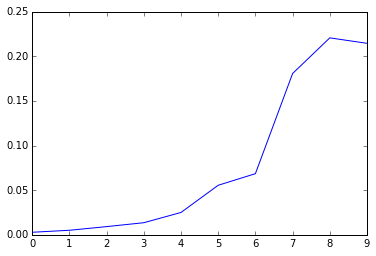
\includegraphics[height=7cm]{timeit/num5_ti2.png}
				\end{center}


			{\bf 3-й способ решения задачи\\}

				В третьем способе решения задачи мы используем поэлементное вместо матричного в 1-ом способе.

				Скорость выполнения данного способа от размера данных приведен в следующем графике:
				\begin{center}
					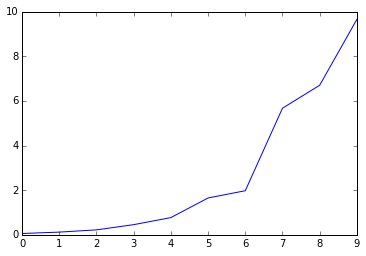
\includegraphics[height=7cm]{timeit/num5_ti3.png}
				\end{center}


			{\bf Сравнение скоростей работы\\}

				Как видно из графиков приведенных выше, самой быстрой оказался 2-й способ решения данной задачи. А самой медленной оказался 1-й способ, что, опять же, является странным, ибо использовался матричное перемножение NumPy. Убедится в этом можно в следующем графике показывающих скорость работы всех методов:
				\begin{center}
					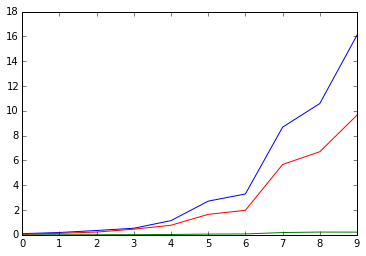
\includegraphics[height=7cm]{timeit/num5_ti123.png}
				\end{center}



		\newpage
		\subsection{Задача 6}

			{\bf Постановка задачи\\}

				Реализовать кодирование длин серий (Run-length encoding). Дан вектор x. Необходимо вернуть кортеж из двух векторов одинаковой длины. Первый содержит числа, а второй - сколько раз их нужно повторить. \\

			{\bf 1-й способ решения задачи\\}

				Первый способ имеет невектаризованный вариант решения, использующий простой пробег по массиву.

				Скорость выполнения данного способа от размера данных приведен в следующем графике:
				\begin{center}
					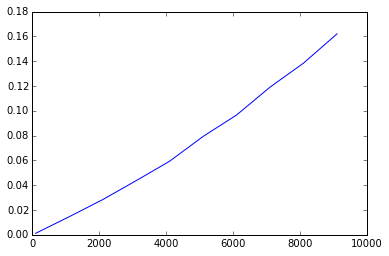
\includegraphics[height=6.5cm]{timeit/num6_ti1.png}
				\end{center}


			{\bf 2-й способ решения задачи\\}

				Во втором способе используются встроенные функции NumPy

				Скорость выполнения данного способа от размера данных приведен в следующем графике:
				\begin{center}
					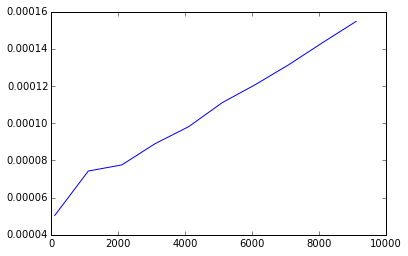
\includegraphics[height=6.5cm]{timeit/num6_ti2.png}
				\end{center}


			{\bf 3-й способ решения задачи\\}

				В третьем способе решения задачи мы используем гибрид NumPy функций и циклы.

				Скорость выполнения данного способа от размера данных приведен в следующем графике:
				\begin{center}
					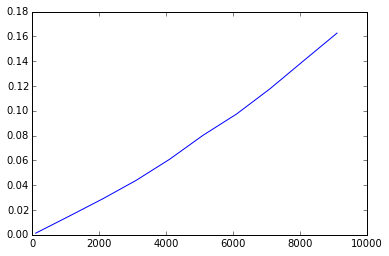
\includegraphics[height=7cm]{timeit/num6_ti3.png}
				\end{center}


			{\bf Сравнение скоростей работы\\}

				Как видно из графиков приведенных выше, самой быстрой оказался 2-й способ решения данной задачи. А 1-й и 3-й способы задачи работают за одинаковое время. Убедится в этом можно в следующем графике показывающих скорость работы всех методов:
				\begin{center}
					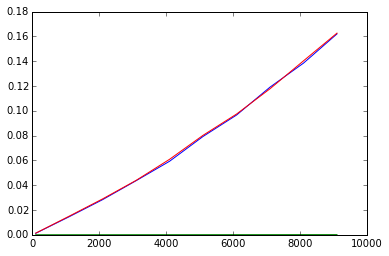
\includegraphics[height=7cm]{timeit/num6_ti123.png}
				\end{center}



		\newpage
		\subsection{Задача 7}

			{\bf Постановка задачи\\}

				Даны две выборки объектов - X и Y. Вычислить матрицу евклидовых расстояний между объектами. \\

			{\bf 1-й способ решения задачи\\}

				Первый способ имеет невектаризованный вариант решения, использующий двойной цикл и некоторые функции NumPy.

				Скорость выполнения данного способа от размера данных приведен в следующем графике:
				\begin{center}
					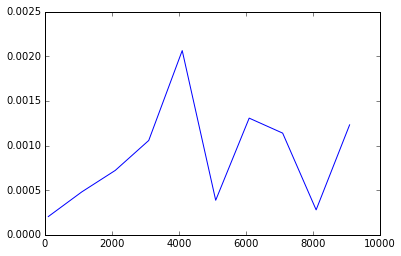
\includegraphics[height=7cm]{timeit/num7_ti1.png}
				\end{center}


			{\bf 2-й способ решения задачи\\}

				Во втором способе используются встроенные функции NumPy

				Скорость выполнения данного способа от размера данных приведен в следующем графике:
				\begin{center}
					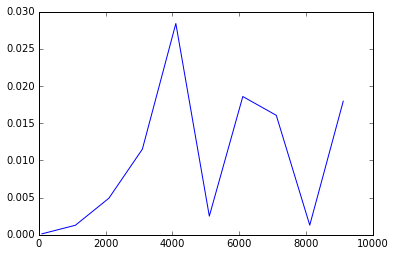
\includegraphics[height=7cm]{timeit/num7_ti2.png}
				\end{center}


			{\bf 3-й способ решения задачи\\}

				В третьем способе решения задачи мы используем тройной цикл без использования функций для массивов NumPy.

				Скорость выполнения данного способа от размера данных приведен в следующем графике:
				\begin{center}
					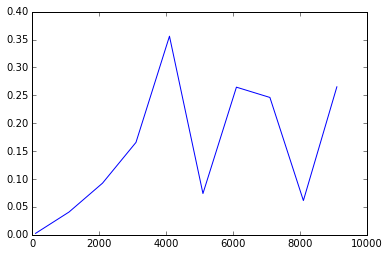
\includegraphics[height=7cm]{timeit/num7_ti3.png}
				\end{center}


			{\bf Сравнение скоростей работы\\}

				Как видно из графиков приведенных выше, самой быстрой оказался 1-й способ решения данной задачи. Это единственный случай, когда функции NumPy работают медленнее обычного прохода по матрице. А 2-й способ явно оказался быстрее 3-го способа. Убедится в этом можно в следующем графике показывающих скорость работы всех методов:
				\begin{center}
					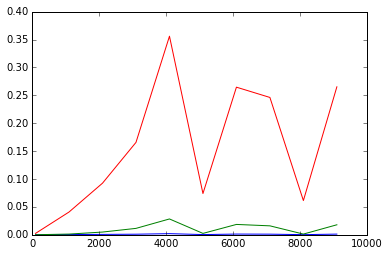
\includegraphics[height=7cm]{timeit/num7_ti123.png}
				\end{center}



		\newpage
		\subsection{Задача 8}

			{\bf Постановка задачи\\}

				Реализовать функцию вычисления логарифма плотности многомерного нормального распределения Входные параметры: точки X, размер (N, D), мат. ожидание m, вектор длины D, матрица ковариаций C, размер (D, D). \\

			{\bf 1-й способ решения задачи\\}

				Первый способ решается благодаря использованию встроенной в SciPy функции.

				Скорость выполнения данного способа от размера данных приведен в следующем графике:
				\begin{center}
					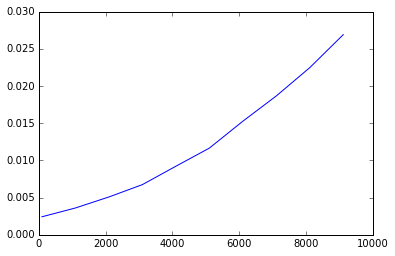
\includegraphics[height=7cm]{timeit/num8_ti1.png}
				\end{center}


			{\bf 2-й способ решения задачи\\}

				Во втором способе используются встроенные функции NumPy

				Скорость выполнения данного способа от размера данных приведен в следующем графике:
				\begin{center}
					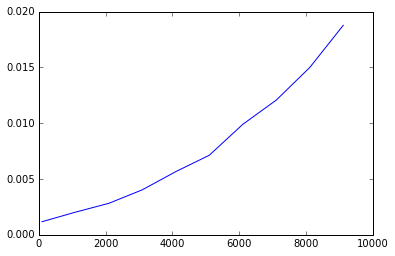
\includegraphics[height=7cm]{timeit/num8_ti2.png}
				\end{center}


			{\bf 3-й способ решения задачи\\}

				В третьем способе решения задачи мы используем гибрид NumPy функций и циклы.

				Скорость выполнения данного способа от размера данных приведен в следующем графике:
				\begin{center}
					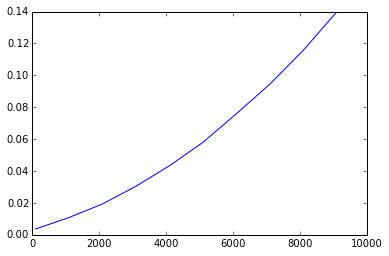
\includegraphics[height=7cm]{timeit/num8_ti3.png}
				\end{center}


			{\bf Сравнение скоростей работы\\}

				Как видно из графиков приведенных выше, самой быстрой оказался 1-й способ решения данной задачи. Т.е. встроенная в SciPy функция работает немного медленнее, т.к. в нем идут всякого рода проверки и исключения. В следующем графике приведен график скоростей работы всех методов:
				\begin{center}
					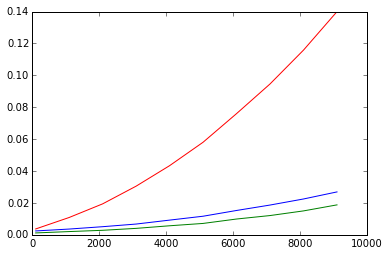
\includegraphics[height=7cm]{timeit/num8_ti123.png}
				\end{center}



		\newpage
		\subsection{Тест на совпадение ответов}
			Запустим модуль с тестами 10 раз и проверим, будут ли ответы положительными

			\begin{center}
				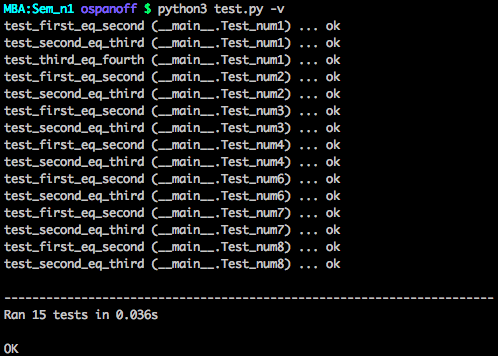
\includegraphics[height=5cm]{test/1.png}
				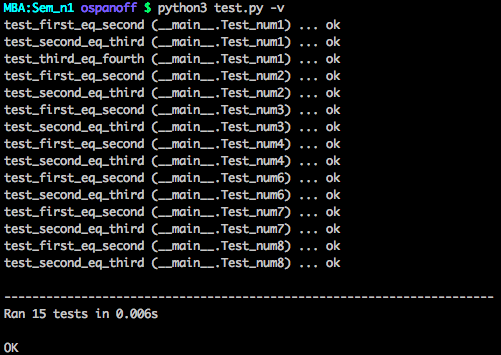
\includegraphics[height=5cm]{test/2.png}
			\end{center}

			\begin{center}
				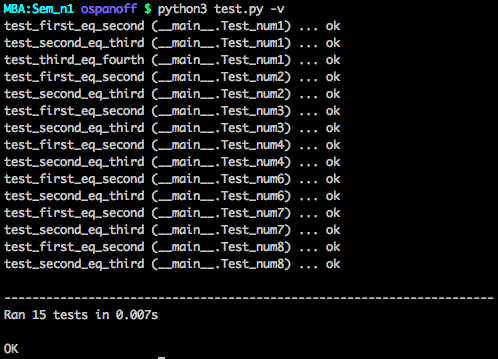
\includegraphics[height=5cm]{test/3.png}
				\includegraphics[height=5cm]{test/4.png}
			\end{center}

			\begin{center}
				\includegraphics[height=5cm]{test/5.png}
				\includegraphics[height=5cm]{test/6.png}
			\end{center}

			\begin{center}
				\includegraphics[height=5cm]{test/7.png}
				\includegraphics[height=5cm]{test/8.png}
			\end{center}

			\begin{center}
				\includegraphics[height=5cm]{test/9.png}
				\includegraphics[height=5cm]{test/10.png}
			\end{center}

			Как можно видеть из картинок, ответы положительные, т.е. выводы всех методов в каждой задаче равны.

			Но в данном тесте не участвует задача 5, т.к. выходные данные (оттенки серого) немного отличаются в библиотечном варианте и в ручном варианте.



	\newpage
	\section{Заключение}
		На протяжении данной работы мы протестировали и перепробовали многие методы решения задач. Некоторые оказались хорошими, некоторые очень долгими и неоптимальными. Но, как показала статистика и графики, лучше всех по скорости работы справляются функции из библиотеки NumPy. В частных случаях, библиотеки справлялись хуже (незначительно), но это можно объяснить тем, что входные данные, перед тем как использоваться, проверяются на валидность. Таким образом, можно сделать вывод, что библиотеки из NumPy в большинстве случаев, можно использовать не сомневаясь.



	\newpage
	% \section{Библиография}
	\begin{thebibliography}{9}
		\bibitem{numpy_and_numpy}
			Документация NumPy \& SciPy \href{http://docs.scipy.org/doc/}. Режим доступа: \href{http://docs.scipy.org/doc/}{http://docs.scipy.org/doc/}
	\end{thebibliography}

\end{document}
